%\documentclass[twocolumn]{article}
\documentclass[journal]{IEEEtran}
\usepackage{blindtext}
\usepackage{amsmath, mathrsfs, tikz, caption, amssymb, fancyhdr, 	epstopdf, geometry, hyperref, float, siunitx}
\usepackage{graphicx}
\usepackage{caption}
\usepackage{multicol}
\usepackage{subcaption}
\usepackage[sort,nocompress]{cite}
\usepackage{matlab-prettifier}
\usepackage{minted}
%\usepackage{titling}

\hypersetup{
	colorlinks = true,
	linkcolor = {blue},
	linkbordercolor = {white}
}

\geometry{a4paper, portrait, margin=1in}

\numberwithin{equation}{subsection}
\numberwithin{figure}{subsection}
\captionsetup{labelfont=bf}
\graphicspath{ {figures/} }

\usepackage{listings}

\renewcommand{\thesubsection}{\thesection.\alph{subsection}}
\newcommand{\lapL}[1]{\mathscr{L}\{#1\}}
\setlength{\parindent}{0pt}

\pagestyle{fancy}
\fancyhf{}
\setlength{\headheight}{25pt}
\lhead{Do a Flip}
\rhead{MTRX5700 Major Project}
\rfoot{\thepage}

%opening

\begin{document}

\title{Do a Flip: the Dancing Drone}
\author{Neill~Foweraker~\textit{430225437}, Angus~Mitchell~\textit{440246554}, Xue~Yin~Zhang~\textit{440305585}}
\maketitle

%\tableofcontents
%\listoffigures
%\newpage


\begin{abstract}
The aim of our project is to create a dancing drone using the Parrot AR Drone 2.0 Power Edition. In order to set ourselves some challenges with our dancing drone, we decided on a set features that we would want our drone to be capable, including: (1) executing dance moves in synchronisation with music as amplified through a speaker, (2) implementing sound processing to detect beats within the music, as well as different sections and moods within the piece of music to determine which dance move to next execute, (3) confining the drone to a volume of space within which it may dance and move, so as to avoid obstacles, (4) responding to a song of the user's choosing by performing real-time sound processing. These four sets of features and challenges form the scope of our dancing drone project.
\end{abstract}
\section{Background}

Whilst a dancing drone is not a completely new idea, they are poorly documented in academic literature, likely because of its limited usefulness outside of a fun and whimsical display of drone technology. We did, however, take to YouTube to find an abundance of dancing drone videos which we used as inspiration for what we could aim to achieve, the most impressive being Intel's swarm of 500 drones, a custom drone which Drexel University created for a dance company called Parsons Dance, and Parrot's own demonstration of the Bebop at a drone convention.\\

%% put these either as hyperlinks or as references
% insert hyperlink for Intel: https://www.youtube.com/watch?v=aOd4-T_p5fA
% insert hyperlink for Drexel: https://www.youtube.com/watch?v=SsPZZrXBUbY
% insert hyperlink for Parrot: https://www.youtube.com/watch?v=A_3UifFb45Y

If we split our dancing drone problem into a sound processing problem and a drone control problem, there is much more previous work which we can piggy-back off of, both in the academic space as well as in drone hobbyist culture.\\

Sound processing is central to creating an intersting and aesthetically pleasing dance. This involves finding a song's tempo or beat, and determining what type of dance move is appropriate. The main requirement for tempo detection is to determine when a beat is in the music, ultimately allowng the drone to time its dance moves. To determine which dance move to execute, a machine learning approach was taken. The objective of this is to split the song into several distinct sections, and to determine what dance is appropriate in each section. 



While parrot provides a SDK for controlling the ARDrone.2, however this was only used as a reference. An alternative
implementation of drone control, the python library `PS-Drone' was used.

\section{Experimental Design} % section could also be called experimental set-up

\subsection{Program Design}
%%NEILL: paragraph or two about overall system architecture, e.g. what runs on-board the drone, what's off-board, what's being done runtime, what's been pre-processed (e.g. clustering is trained beforehand)

The dancing drone software solution is broken down into three main modules; the audio module, drone dancer
module and classification module. These modules are all used by a single main script/routine which specifies
what audio to dance to, and the 'mood' of the dancing. All software discussed in this guide ran on a laptop
separate to the drone. While code is able to be compiled to run natively on the ARDrone's ARM processor, the
sensor protocols and actuator control are not documented by Parrot and much of the software running on the
ARDrone is closed source. As Parrot supports controlling the drone over its WiFi network, it was decided that the
code will all be run on a separate device to the drone. Each module discussed below runs asyhcnronously to
prevent from `sleep' functions in the code stalling the music playback or adding a delay before the drone does a
move. By running each module in a different thread, synchronization between music playback and drone movements
can be achieved through event-driven programming rather than looking ahead in the audio file and trying to
predict the next position of the drone in order to make it move in time.\\

\subsubsection{Audio Module}
The audio module performs pre-processing on a given audio file, or live processing on an audio stream from a
microphone or line in. The audio module uses the Aubio library, a free open-source audio processor. The Aubio
module is further discussed in the 'Tempo Detection' section later in this report. The audio module works
together with the classification module to determine whether the current point in the song is a chorus or a
sparse section. At any point during playback, the current time, bpm and section label (chorus or sparse) can be
retrieved. In the case of live audio processing, the current time is not relevant as beat/onset events are fired
when detected. \\

For live processing, the audio module delays outgoing audio (in the case of using line-in). In the case of
reading audio from a microphone, no lookahead can be implemented as the audio cannot be delayed as it is coming
from an external, audile source. Line-in audio is able to be delayed as it is played by the audio module, and is
not audible unless the line-in is configured to be so in the sound settings of the computer being used. Lookahead
was needed for accurate bpm representation of live audio where the bpm varies over the song or between sections.
The reasons for this are outlined in the 'Tempo Detection' section further in this report, where the limitations
of the Aubio library are discussed. The code behind the audio module is viewable at \eqref{code:play_song.py}\\

The audio module also handles synchronization of events that should be performed to the beat, or on the onset of
a beat. Function pointers can be given to the audio module to be executed when it detects a beat or onset of a
beat (depending on if the current bpm is regular enough to use). An example of the audio beat event function hook
is shown below, with input generated by clapping next to the microphone.\\

\begin{figure}[h]
    \centering
    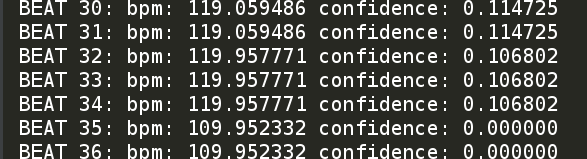
\includegraphics[scale=0.3]{BEAT}
    \caption{The audio beat event firing, triggered by clapping near the microphone. Notice that when the bpm
    changes significantly, the bpm confidence drops to 0.}
\end{figure}

\subsubsection{Drone Dancer Module}
The drone dancer module is responsible for all physical movements of the drone. One of the main limitations of
the ARDrone.2 encountered was the internal command-queue behaving inconsistently. According to Parrot's
documentation, when using the in-built animations of the drone (backflip, bob nose down etc.), the animation code
and duration must be specified in order to let the drone know how long to wait until attempting to perform the
next animation. The drone did not always behave consistently and wait for the specified duration between moves,
and sometimes required strange values to work. An example of this is performing flips, a duration of 15ms must be
given (as opposed to 1000ms or 6s as specified in Parrot's SDK examples) and then a 'hover' command sent 0.45s
later. Operations such as this are abstracted by the drone dancer module, which implements a queue of moves to
do, sleeping for the appropriate amount of time when each one is sent. At any time dancing can be paused and
resumed without affecting the moves in the queue.\\

The move queue is one of the main motivators for making the dancing drone solution multi-threaded. As the drone
dancer module runs in its own thread, any sleeps performed within it do not affect the audio playback or
operation of the rest of the program.\\

The drone dancer contains definitions for each kind of move the drone can do, and some functions that when called
repeatedly dance in a certain 'mood'. Each move takes varying arguments, for example wiggling to a certain
frequency, or bobbing in a different direction each time the same function is called. These parameters can be
given manually or can be generated automatically by the drone dancer class using the current bpm or onset given by the
audio module. The drone's dancing is generally driven by a function being called on the beat or on the onset of a
beat by the audio module, as discussed in the previous section. For the code behind the drone dancer module, see
\eqref{code:drone_dancer.py}.\\

The drone dancer class is also responsible for navigation of the drone. Using a separate thread, the navigation
data is constantly read in from the drone. If a roundel is detected on the ground, the dancing thread is blocked
until the navigation thread has moved the drone back into a safe location.\\

\subsubsection{Classification Module}
The classification module performs cluster analysis on the last 10 chunks in the current audio stream to
determine whether they are likely to be a chorus or sparse section. The classification module had to be trained before
use, but is able to classify song sections in real time. The operation of the classification module is further
discussed in the sound processing section further in this report. The code behind the cluster module is viewable
at \eqref{code:cluster.py}.\\

\subsubsection{Routine}
The main routine file is what uses all the modules together from their public interfaces in order to make the
drone dance in a certain situation. An example routine file is viewable at \eqref{code:routine_hardstyle.py}.

A data flow diagram showing the high-level communication between each module is shown overleaf.

\onecolumn
\begin{figure*}[h]
\begin{tikzpicture}

\draw  (-1.5,6.5) circle [radius=1.5] node {Routine / Main};
\draw  (-1.5,2.5) circle [radius=1.5] node {Audio};
\draw  (-7,2.5) circle [radius=1.5] node {Classification};
\draw  (3.5,2.5) circle [radius=1.5] node {Drone Dancer};



\node at (-5.5,5.5) {Audio File};
\draw [->] (-3.0,6.5) -- (-6.0,3.7);


\node at (-3.7,4.5) {Audio File};
\draw [->] (-2.7,5.6) -- (-2.7,3.5);


\node at (-4.2,3) {Song Structure};
\draw [->] (-5.5,2.5) -- (-3,2.5);

\node at (1,3) {\begin{tabular}{c}Beat/Onset\\Events\end{tabular}};
\draw [->] (0,2.5) -- (2,2.5);


\node at (1.5,6) {Dance Style};
\draw [->] (-0.1,6) -- (2.6,3.8);


\node at (6.2,0.5) {Movement Commands};
\draw [->] (3.5,1) -- (3.5,-0.5);

\draw  (2,-0.5) rectangle (5,-2) node[pos=.5] {Drone};
\end{tikzpicture}
\caption{High level Data Flow Diagram of the dancing drone solution.}
\end{figure*}

\begin{multicols}{2}
\twocolumn

\end{multicols}
\clearpage

% todo neill


\subsection{Sound Processing}

%%ANGUS: for you to discuss how we achieved what's been specified in the intro - make subsubsections for like brief description of how we're using aubio, beat detection, clustering, etc...

%% fix the intro/background if you feel inaccurately describes the sound processing bits (doesn't need to be too detailed in the intro/background) - your time to shine is here and in section 4

The objective of the sound processing module was to extract information from the song, in both live, and non live cases. Non live processing involves parsing the entire song before it is played, while the live case involves playing and processing the song 'on-the-fly'. Processing in the non live case is significantly easier, as sufficient time is available for calculations, and context of each section in the song can be more easily determined. This module extracted the tempo of the song and attempted to classify how the song's sections change throughout. The classification task ultimately decides what type of dance moves or "feel" is appropriate in different sections of the song, while the tempo informs the accurate timing of dance moves.

\subsection{Tempo Detection}
Tempo detection utilised Aubio's tempo and onset detection library. The python library consists of a set of python wrapper classes which can be used to call the C implemented Aubio library. \\
\\
TALK ABOUT SWITCHING BETWEEN ONSET AND TEMPO DETECTION DURING LIVE\\
\\
TALK ABOUT RELIABILITY IN NON LIVE CASE

\subsection{Section Classification}
The goal of classification was to divide the song into several distinct sections which can intuitively be called "intro", "verse", "chorus" or "instrumental". Automating this process posed a significant challenge. The approach that was taken was a machine learning approach, using a set of features in the song to classify the type of each section of the song. \\
\\
The first step in this process was to extract some meaningful features from the song at each time step. It was determined that the best way to achieve this was to use MFCC (mel-frequency cepstral coefficients.) This is a method of feature extraction often used in genre classification and speech recognition (1)(2). This technique yields a set of meaningful features that are much less expensive to process than the raw sound samples. Use of a down sampled version of the song as a feature vector was considered, however, doing this would result in the loss of high frequency components and would still be computationally expensive. The "scikit.talkbox" python library was used to extract the MFCCs. This module allowed a maximum of 40 MFCCs for each song "chunk" that was processed. This maximum value was chosen, in order to yield a maximally detailed feature vector to the following step.\\
\\
The next step in this process involved reducing the set of 40 dimensional feature set down to a lower dimension for processing and visualisation or clusters. PCA was applied, a process which reduces high dimensional features down by projecting less deterministic (or less independent) features onto the axis of the more independent features. The result was a set of two features, which could be plotted against the third features, which was time. \\
\\
After this, a simple means shift clustering algorithm was applied to separate out song "sections". The Algorithm was applied to the three dimensional (two frequency dimensions plus one time dimension) features\ vector to find distinct sections in the song. It should be noted that this algorithm is merely "clustering" the song chunks according to their frequency characteristics and their time in the song - it is not performing classification. Sections in the song tend to share distinct frequency components, and are also grouped together in time (i.e. if the current section is a sparse instrumental section, it is likely that the sections immediately after and before are also sparse instrumental sections.)\\
\\
The final step was to compare the extracted cluster centroids to known cluster centroids of different song sections such as "sparse", "verse", "rock chorus" and "EDM chorus". This step allows the sections to be classified in terms of their similarity to the sample song sections. 



(1) http://cs229.stanford.edu/proj2009/RajaniEkkizogloy.pdf
(2)	http://cs229.stanford.edu/proj2011/HaggbladeHongKao-MusicGenreClassification.pdf
% todo:
% clustering for chorus / sparse
% bpm detection with aubio, and beat onset
% processing live by chunk, preprocessing
% live audio via aux in or reading from a file


\subsection{Latency Management}

%%NEILL: multithreading stuff, how dance moves are synchronised with the music, peculiarities with the drone software, how to specify the length of moves, etc...
%I don't know if you wanna about how some of the dance moves were hardcoded ^_^"
% optional: live stuff, like how there is a bit of latency before the drone starts moving because it takes a few beats to confirm a high enough confidence of bpm

Latency is an important aspect of the dancing drone solution, as the drone must perform a move suitably fast in
order to appear visually pleasing and in time with the music. Experimentally, we determined that almost all of
the time the drone will begin to respond to a command within 5ms of receiving it, however it can be delayed up to
20ms.

% todo 
% ping drone in the range ~3-5ms but can be up to 20ms


\subsection{Space Confinement}

%%XUEY

\section{Results}

% \subsection{Program Design}

%%NOT SURE IF THIS IS NECESSARY IN RESULTS

\subsection{Sound Processing}

%%ANGUS: for you to discuss how we achieved what's been specified in the intro - make subsubsections for like brief description of how we're using aubio, beat detection, clustering, etc...

%% fix the intro/background if you feel inaccurately describes the sound processing bits (doesn't need to be too detailed in the intro/background) - your time to shine is here and in section 4

Some sound processing modules were implemented sucessfully, while others were not perfect, requiring further refinement. The module that worked very effectivly was beat detection. Switching from tempo to onset detection worked very effectivly for song sections that did not contain a distinct beat, or sections with a changing tempo. Clustering of song sections also worked effectivly, providing a nice way to divide the song up into distinct and useable sections (see figure \ref{fig:cluster_output} and \ref{fig:clustering}). The component that was less affective was the classification. In hindsight, changed could have been made in the classification module to achieve more accurate and useful results. \\
\\
\begin{figure}[H]
      \centering
      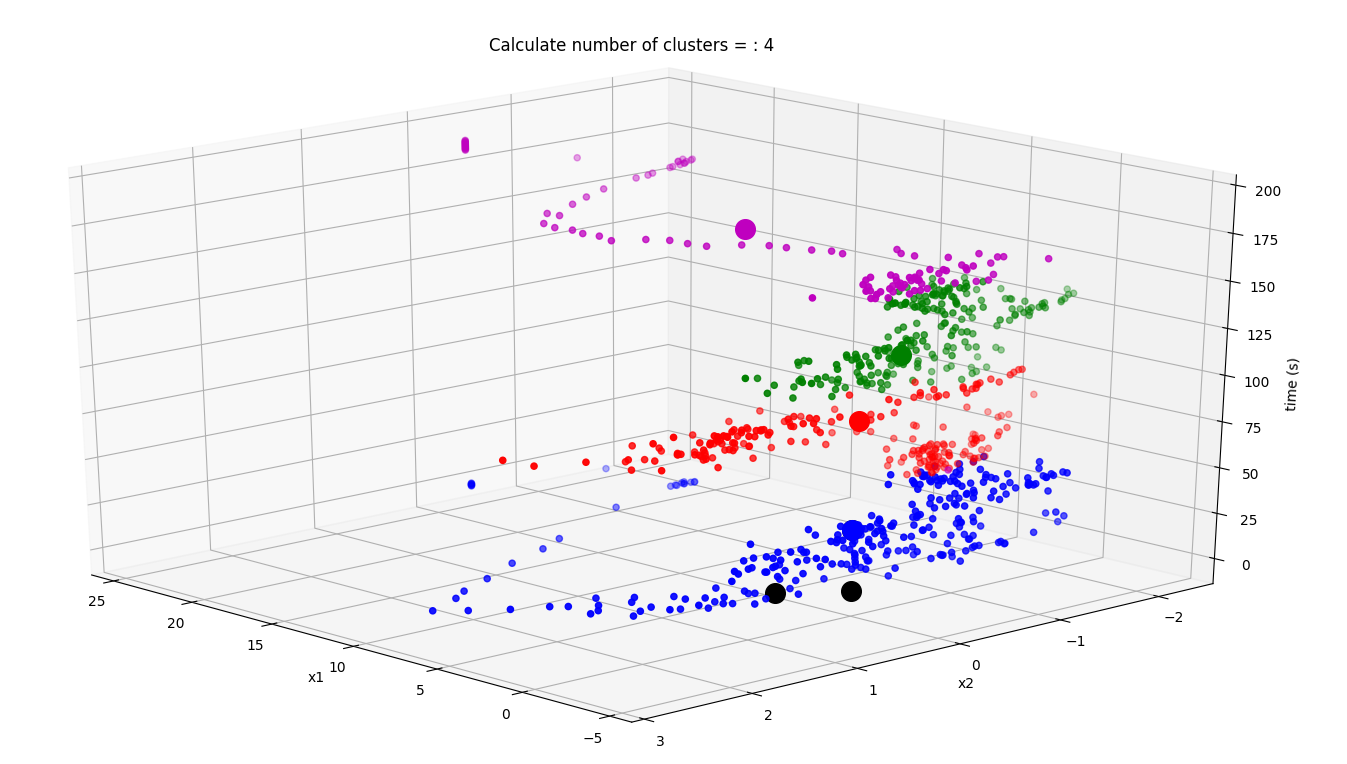
\includegraphics[width=1\linewidth]{clustering.png}
      \caption{Clustering results: the song is divdied into distinct sections. Each colour represents a different cluster, with the cluster centroid represented by the larger markers. x1 and x2 axes represent the reduce feature set, while the vertical axis is time.}
      \label{fig:clustering}
\end{figure}
\begin{figure}[H]
      \centering
      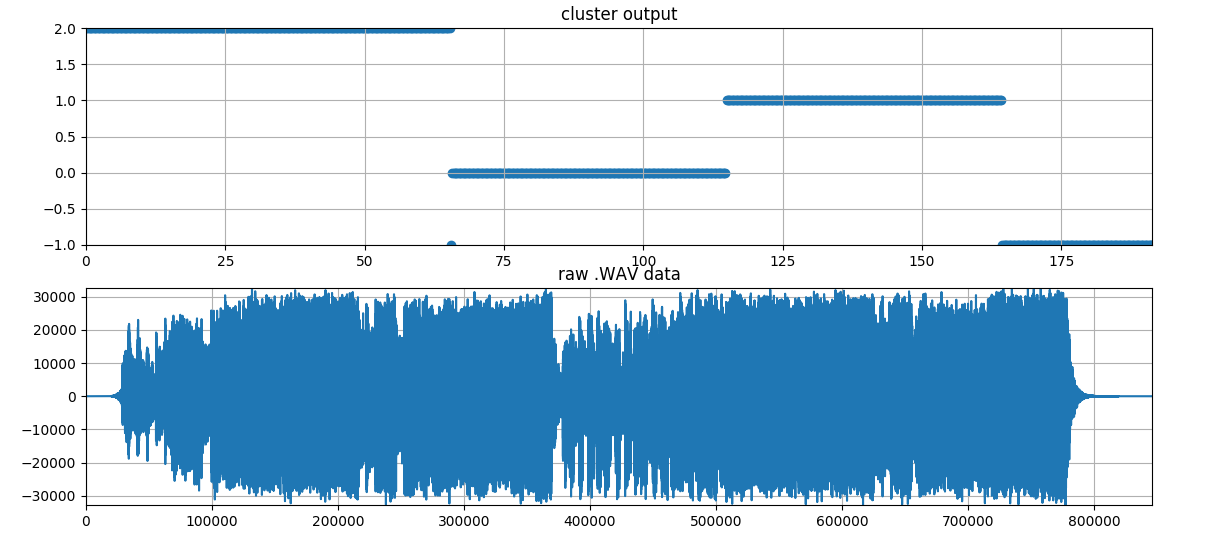
\includegraphics[width=1\linewidth]{cluster_output.png}
      \caption{An alternate view of the clustering results. The cluster number is plotted next to the raw song data.}
      \label{fig:cluster_output}
\end{figure}



\subsection{Latency Management}

% we can talk about system performance by pulling some numbers out of our ass (like numbers in the same ballpark as we were getting when timing how long it took for a packet to send)

% and other things

\onecolumn

\begin{multicols}{2}
\subsection{Space Confinement}

For this module, we successfully configured the drone to receive and decode the navigation data packages that were being sent from the drone to the laptop. The three datasets which were useful to this module are shown in Figure \ref{fig:4c-sample-nav}.

\begin{figure}[H]
      \centering
      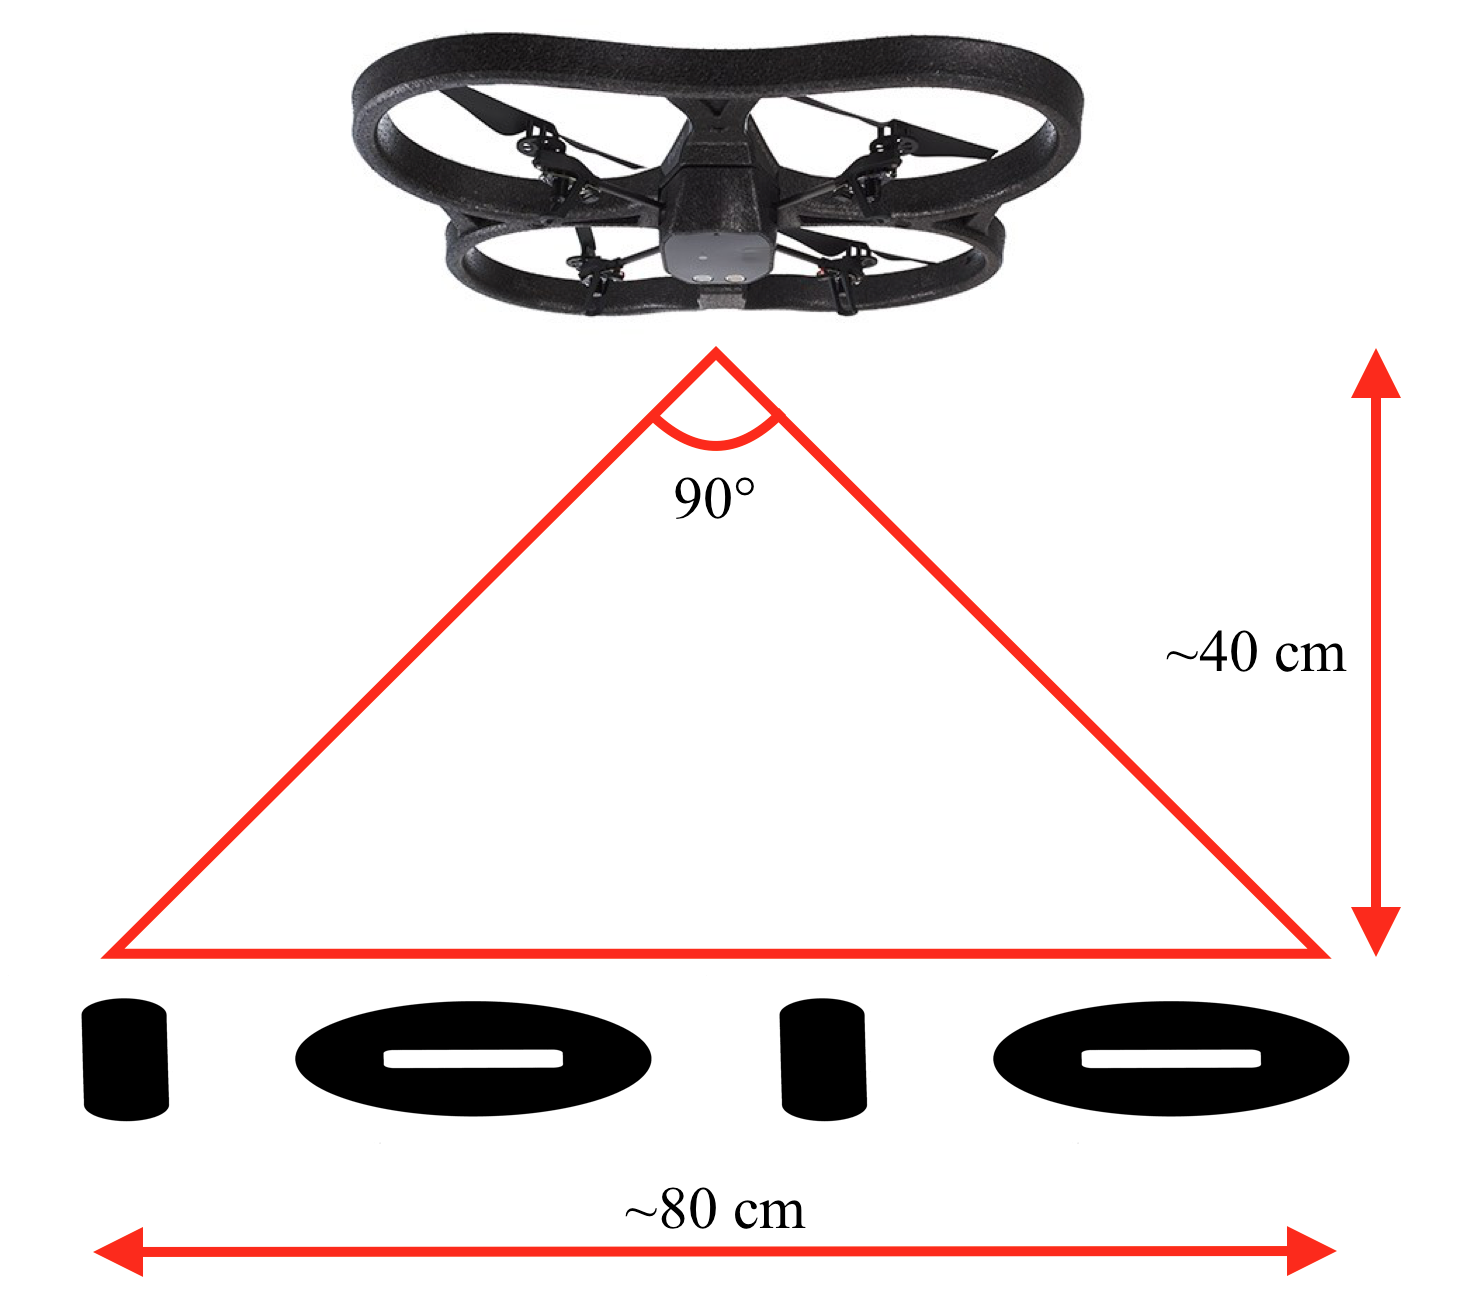
\includegraphics[width=0.8\linewidth]{3d-drone-fov.png}
      \caption{Sample navigation data from the drone when rotating clockwise near a roundel}
      \label{fig:4c-sample-nav}
\end{figure}

The following figure includes a few screenshots from a video where the drone approaches a row of roundels, and then backs away again.

\end{multicols}
\begin{figure}
        \begin{subfigure}[b]{0.25\textwidth}
                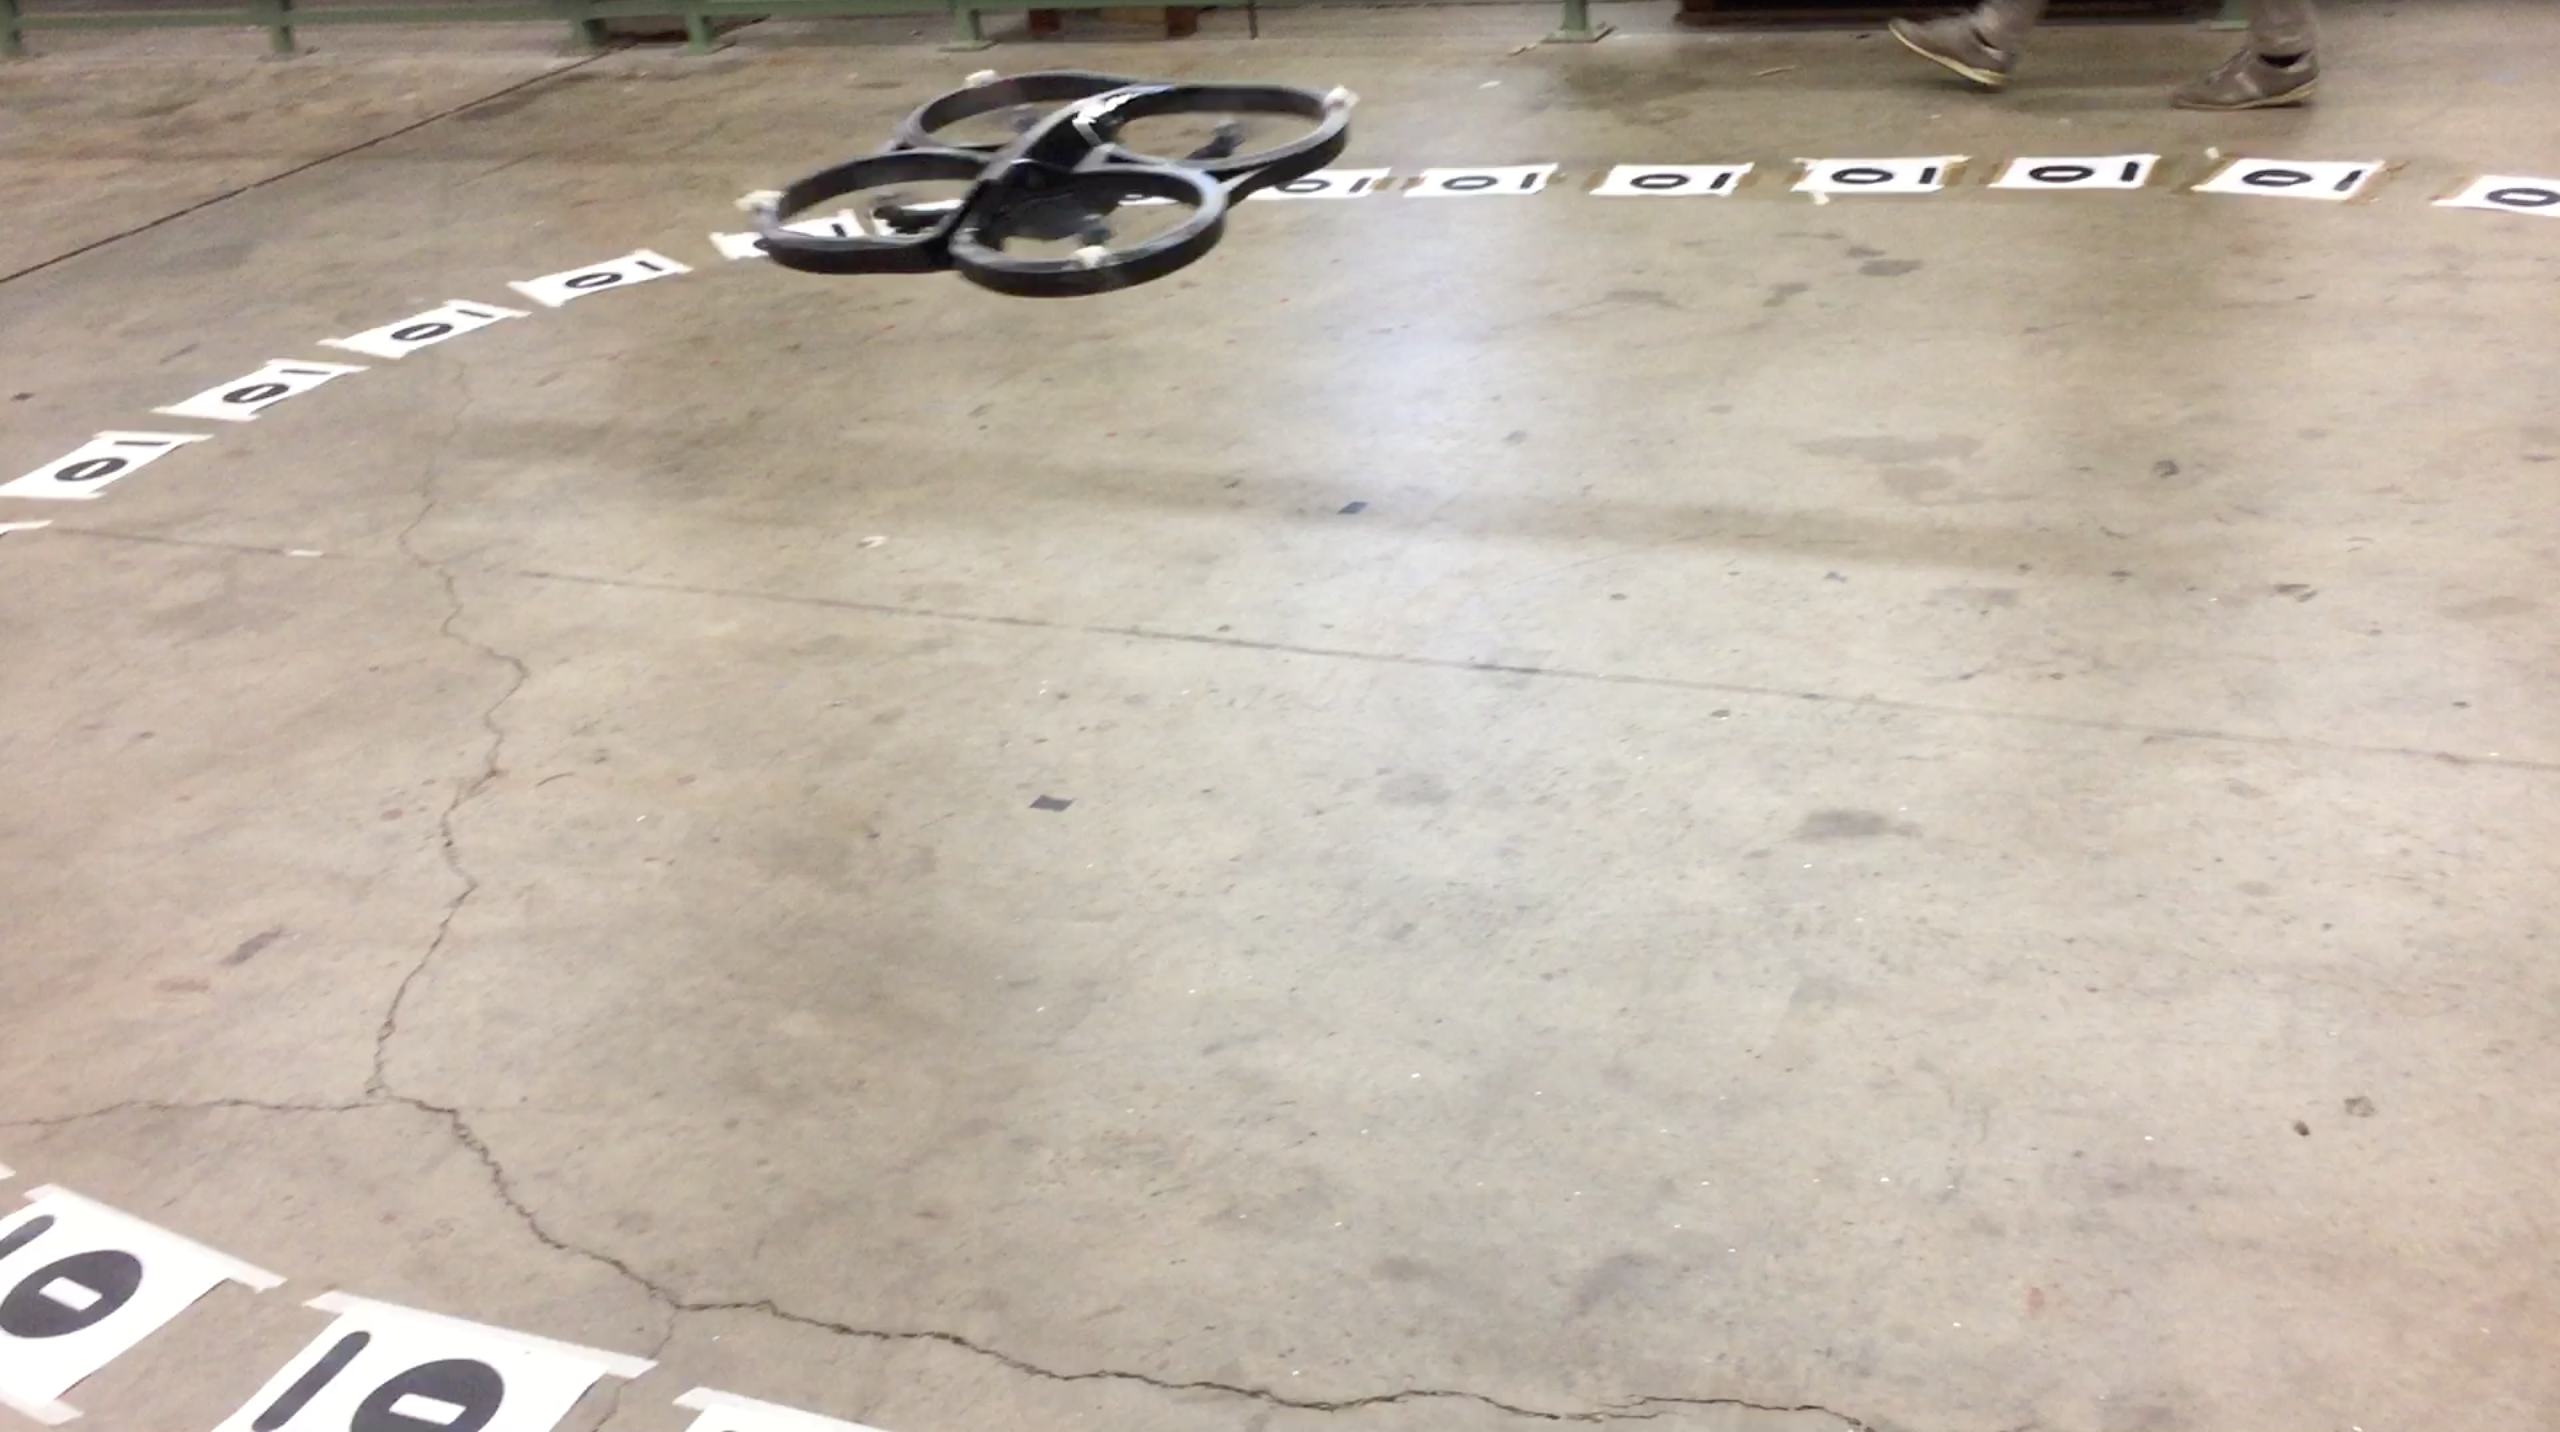
\includegraphics[width=\linewidth]{4c-flying-towards.png}
                \caption{Drone is flying towards the roundel boundary}
        \end{subfigure}%
        \hspace{\fill}
        \begin{subfigure}[b]{0.25\textwidth}
                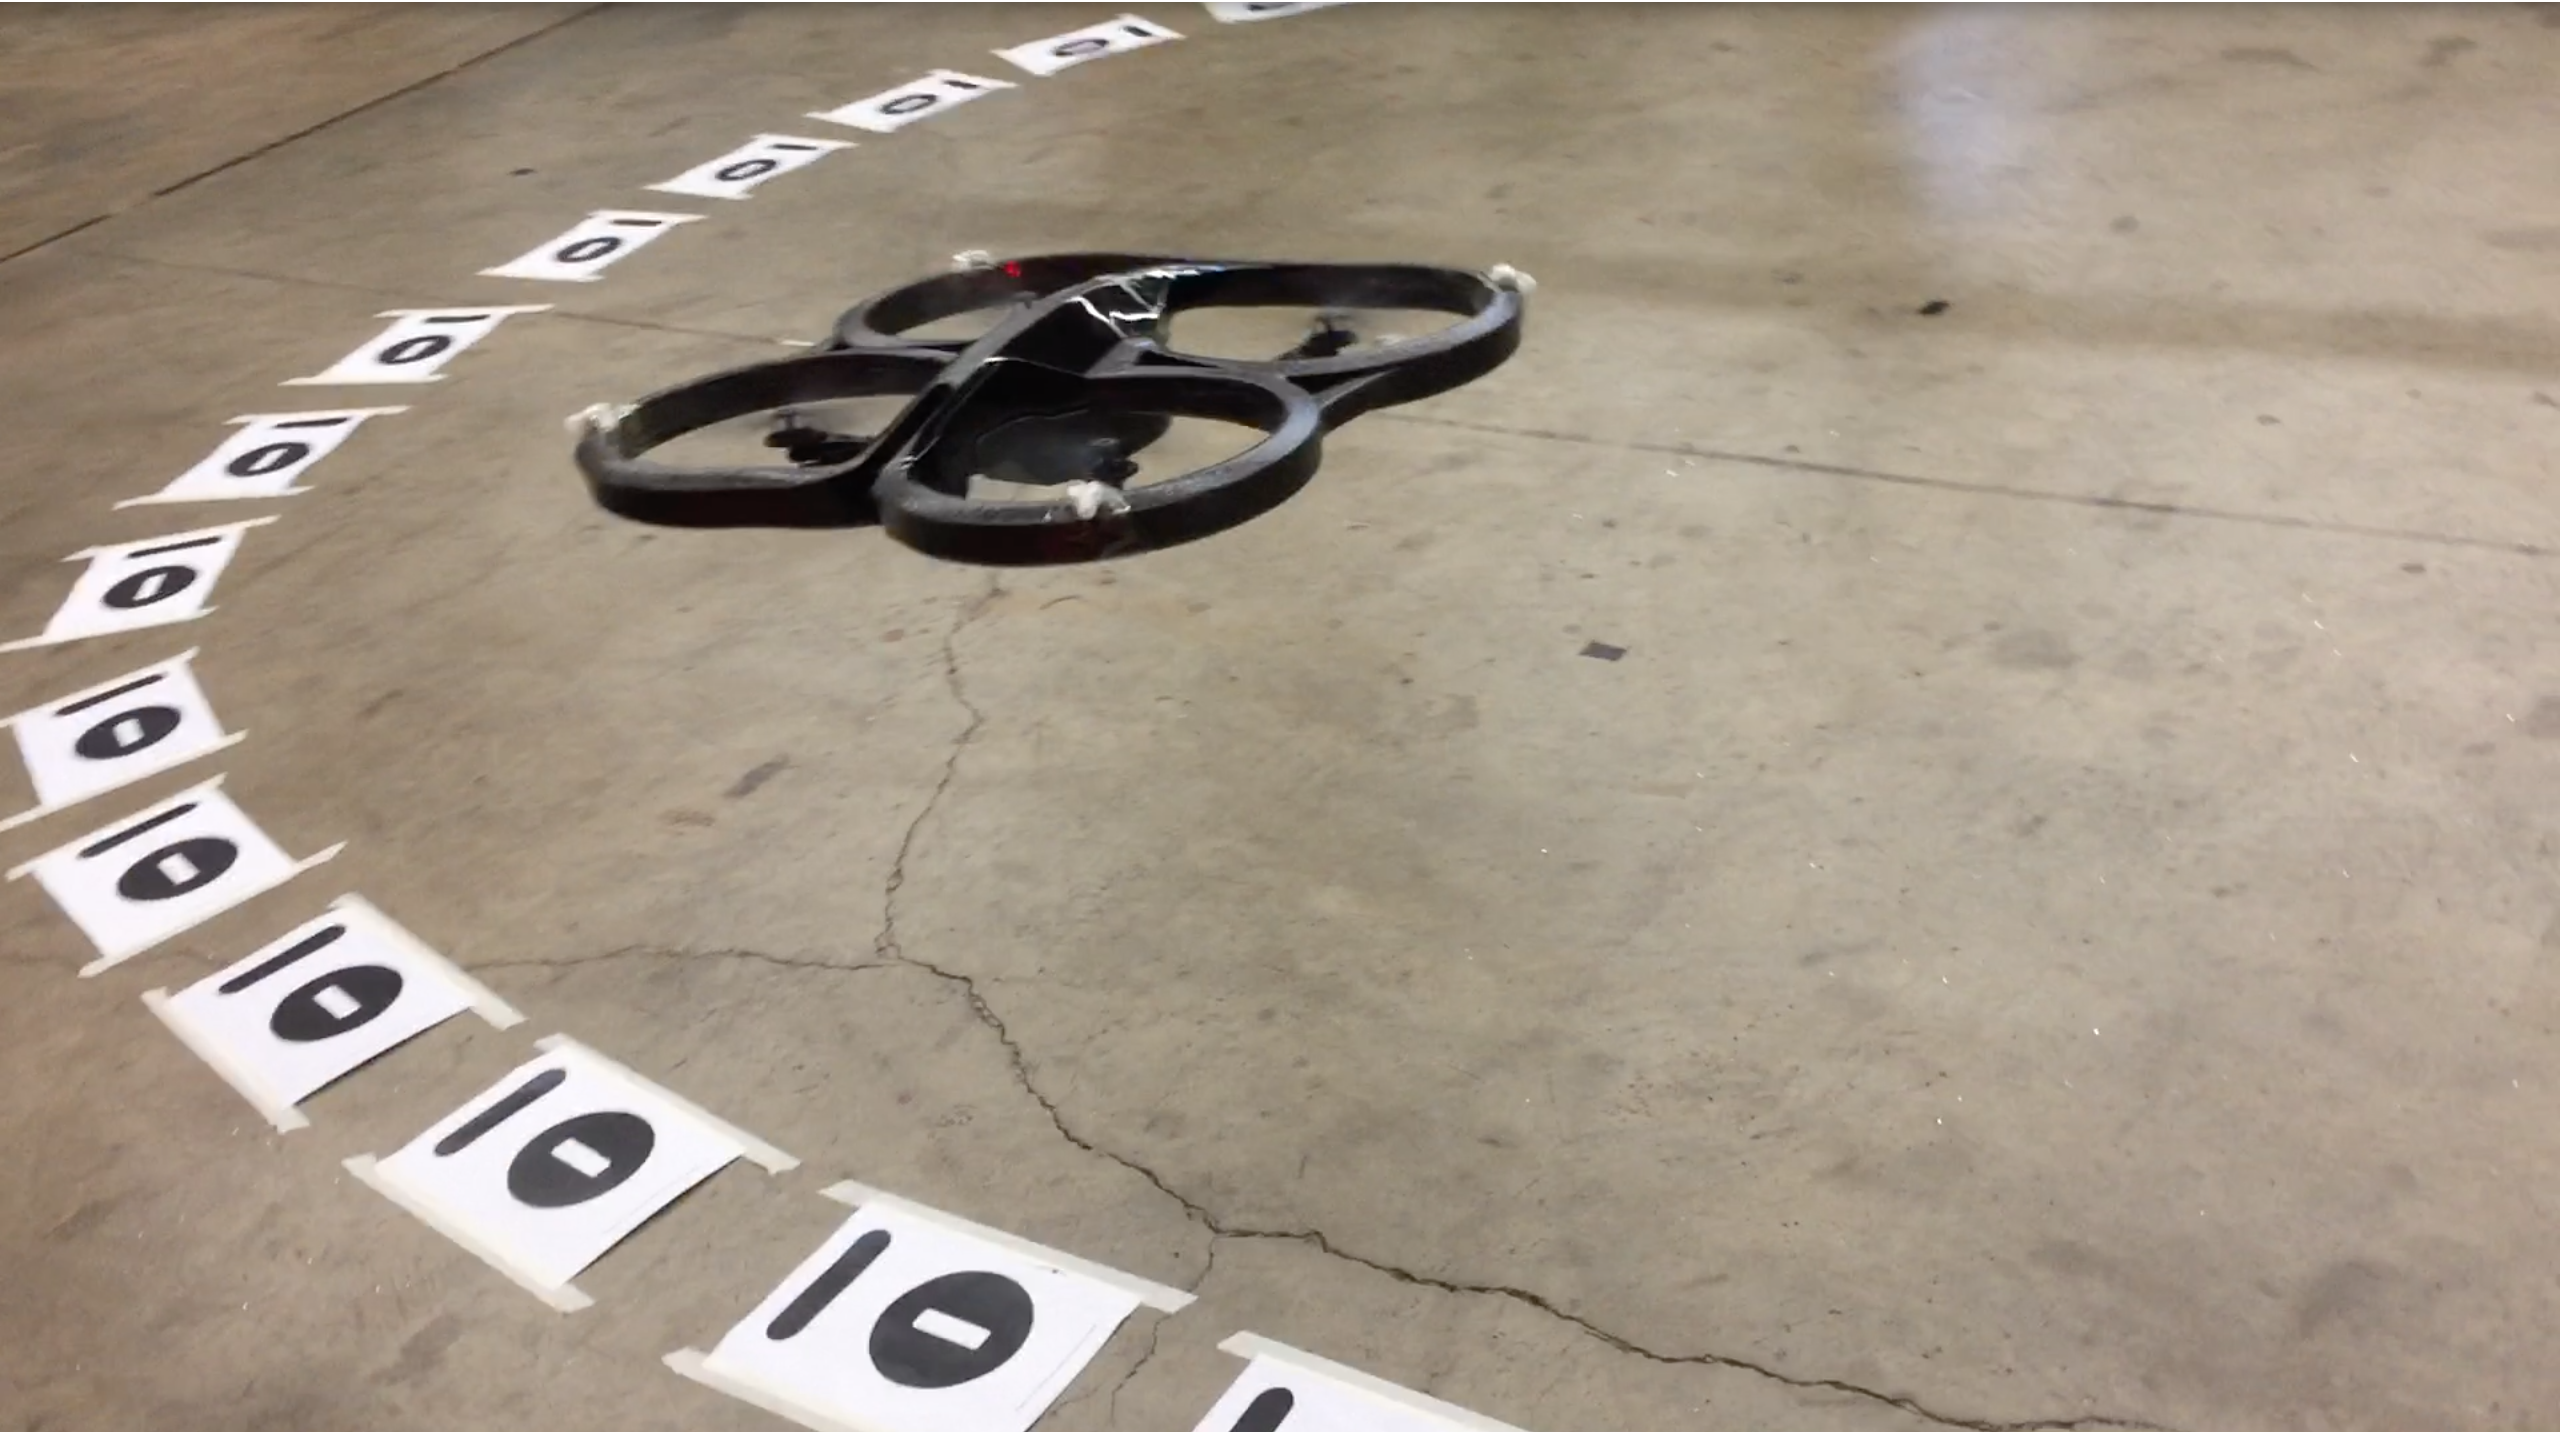
\includegraphics[width=\linewidth]{4c-found-boundary.png}
                \caption{Drone has detected a roundel at the boundary}
        \end{subfigure}%
        \hspace{\fill}
        \begin{subfigure}[b]{0.25\textwidth}
                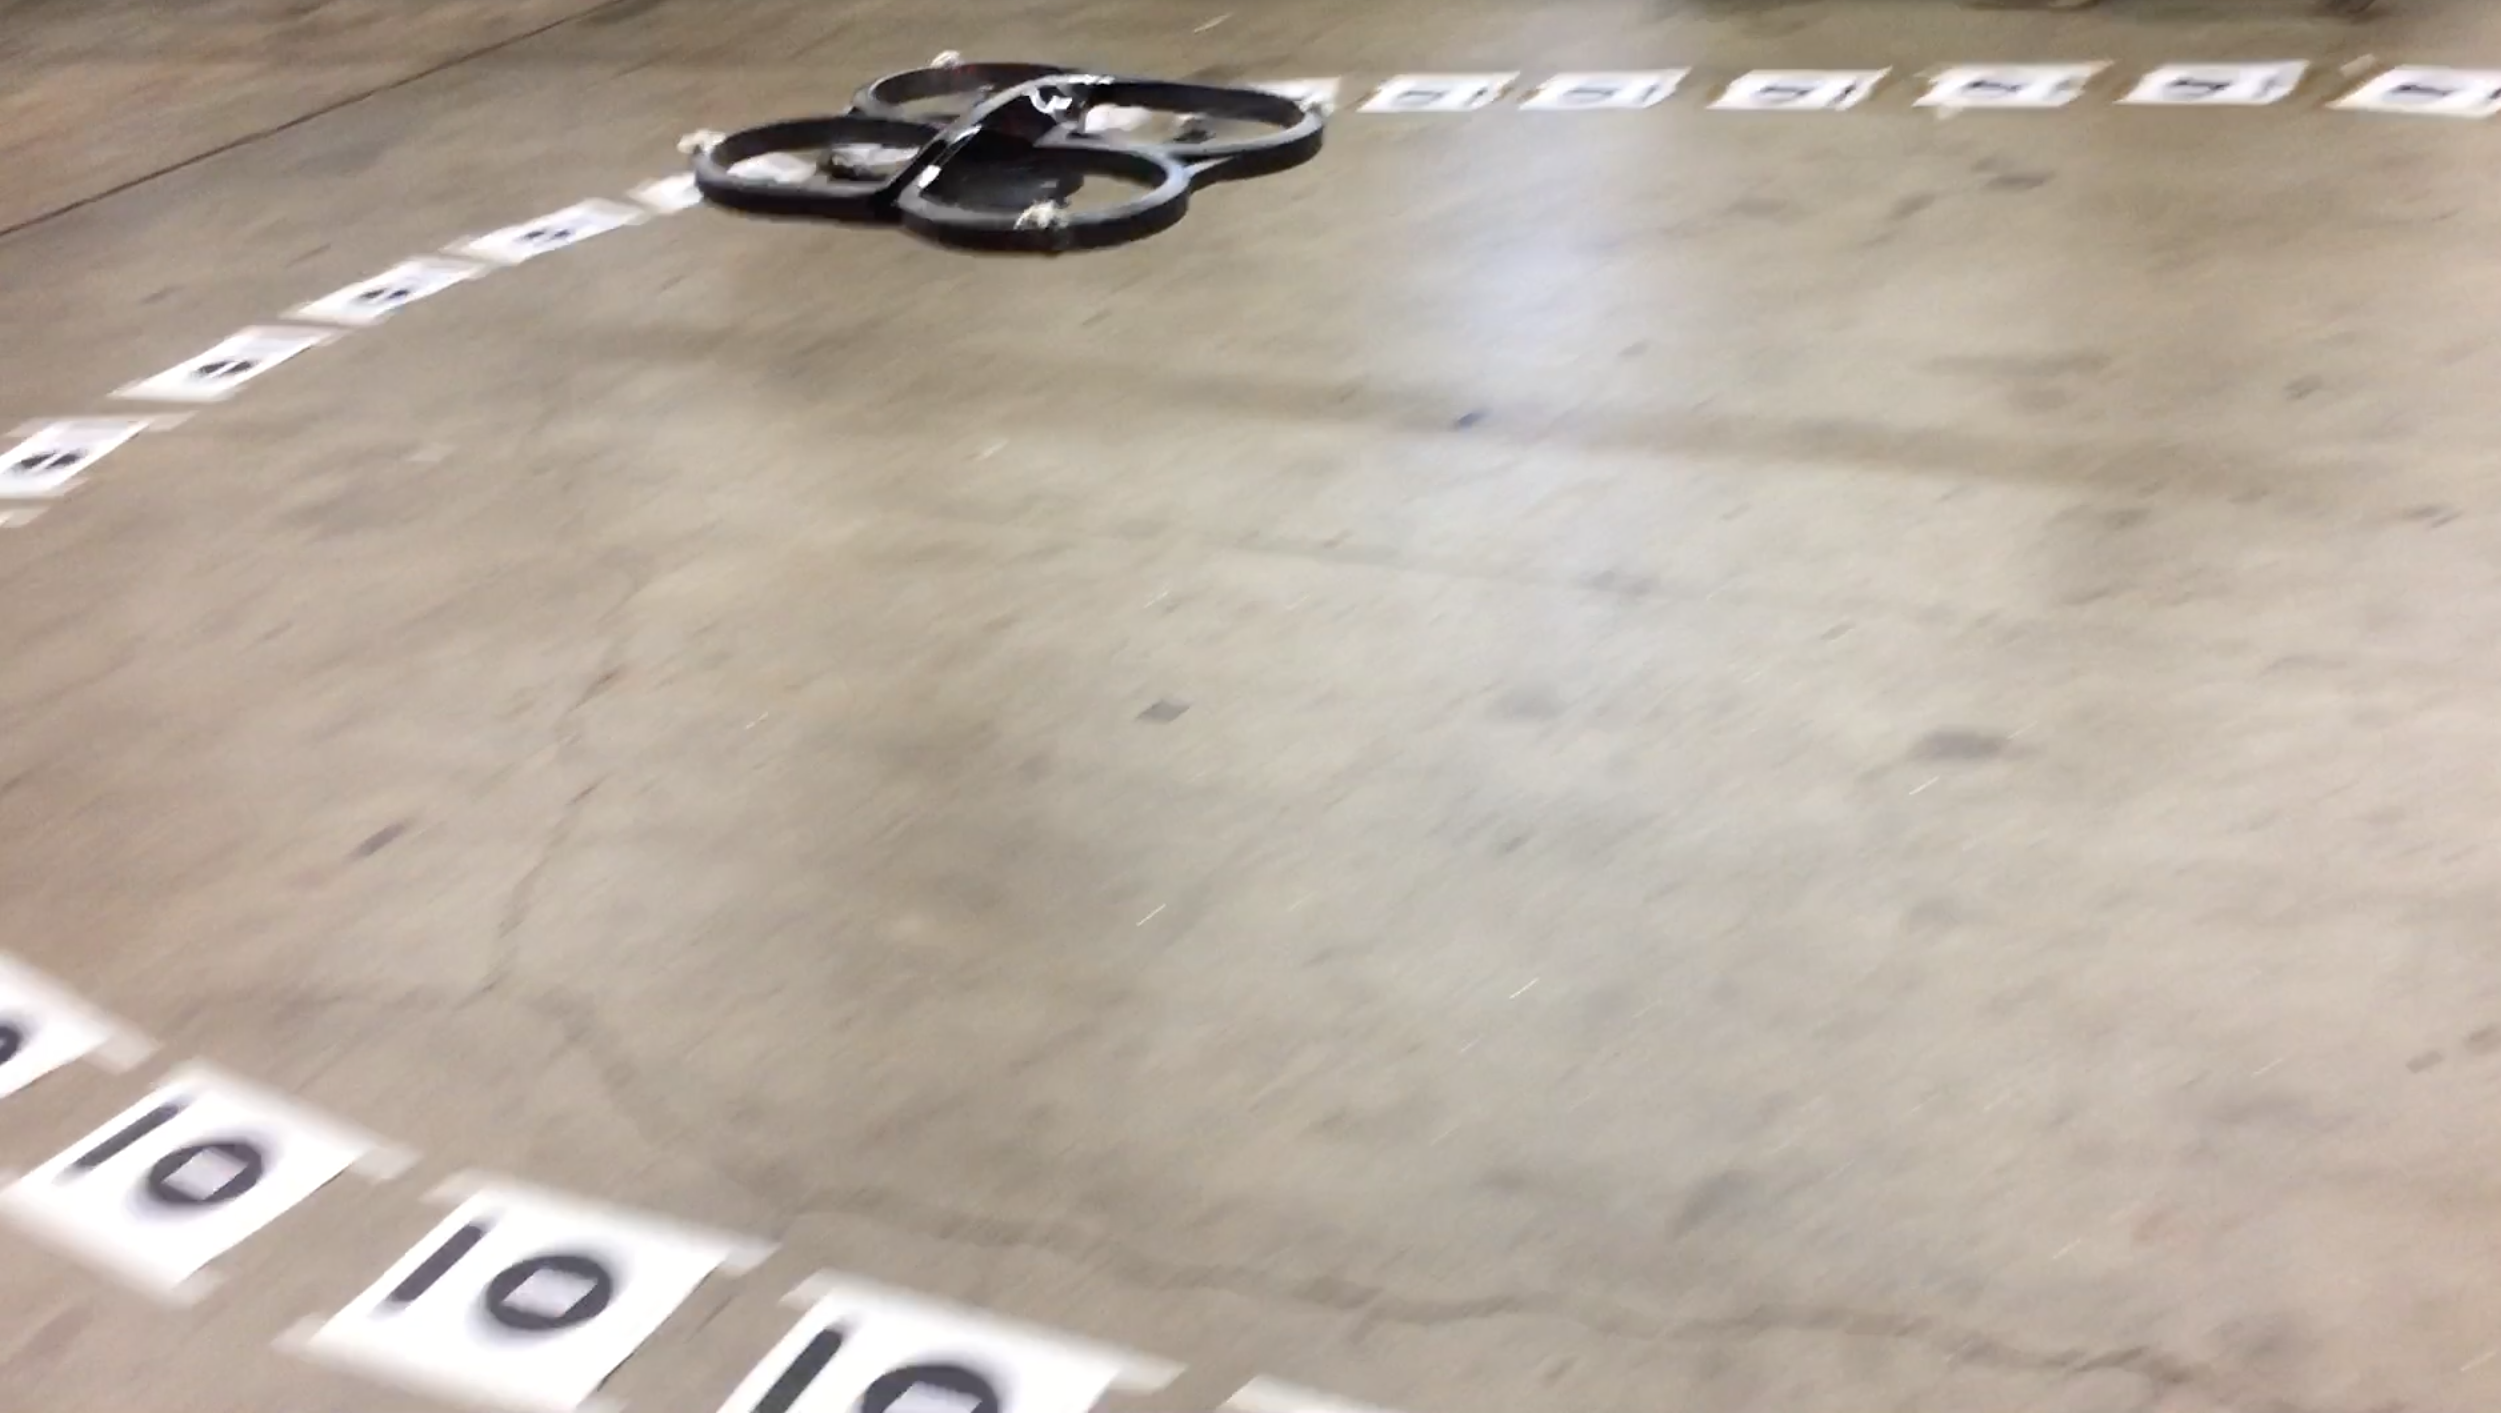
\includegraphics[width=\linewidth]{4c-backing-away.png}
                \caption{Drone is now backing away from the roundel}
        \end{subfigure}
        \caption{Screenshots from a video}\label{fig:4c-video}
\end{figure}
\twocolumn

\section{Discussion}

\subsection{Classification}
A lot was learnt in the design and implementation of the classification module for this project. While the MFCC, PCA and clustering worked well, classification did not work as intended. Some improvements to this module are listed below. 
\begin{itemize}
  \item Use of online database for classification
  \item Implementation of a small multilayer perceptron on training data, using a larger feature vector
  \item Inclusion of a larger set of classes
  \item Use of a larger features vector
\end{itemize}
The use of a three dimensional feature for clustering was on the the main issues. Two frequency based features do not provide enough information for classification to be sucessfully implemented - even if a complex classification method was used.

\section{Conclusions and Future Work} % section could also be called future work

In conclusion, while many of the dancing drones viewable on the internet have a
hard-coded routine, our dancing drone solution was able to meet our goal of dancing to
a previously unknown song. The greatest challenges were using the ARDrone2 animations,
as they operate in a different way than specified in Parrot's SDK. Writing an entire
wrapper class (the drone dancer module) for the drone's physical movements along with
asynchronous operation of each module were required to facilitate our desired behaviour.
In the future, more dance moves and genres could be added, along with bar detection
as well as beat detection. Further audio analysis would also allow for more variation
between moves and different parts of a song, for example using the pitch or key.
For future projects, a smaller, lighter stunt drone would be more suitable.


%\subsection{Future Work}

\newpage
\onecolumn
\section{Appendix}
\subsection{Code Listing}
\subsubsection{Audio Module: play\_song.py}
\inputminted[fontsize=\footnotesize,linenos]{python}{../code/play_song.py}

\newpage
\subsubsection{Drone Control Module: drone\_dancer.py}
\inputminted[fontsize=\footnotesize,linenos]{python}{../code/PS-drone/drone_dancer.py}

\newpage
\subsubsection{Example Drone Semi-Automated Routine: routine\_hardstyle.py}
\inputminted[fontsize=\footnotesize,linenos]{python}{../code/PS-drone/routine_hardstyle.py}

\newpage
\subsubsection{Song Classification: cluster.py}
\inputminted[fontsize=\footnotesize,linenos]{python}{../code/classification/cluster.py}


\bibliographystyle{plain}
\bibliography{biblio}

\end{document}
